\section{Introduction}\label{sec:introduction}
Entity Resolution (ER) is the problem of identifying different entity descriptions that pertain to the same real-world object (e.g., a person, location, or movie)
%in a dataset~
\cite{DBLP:books/daglib/0030287}. ER, as a data cleaning method, increases the quality and, subsequently, the value of the data, which can later be used further for downstream applications, like training a machine learning model. To this end, the available data is processed by end-to-end ER pipelines that consist of 
%Apart from its benefits, though, ER comes with a significant cost. De, ER pipelines involve 
several steps, such as blocking~\cite{DBLP:journals/pvldb/Thirumuruganathan21}, similarity estimation, and clustering~\cite{DBLP:journals/pvldb/HassanzadehCML09,DBLP:journals/vldb/PapadakisETHC23}. Each step
%, in turn, 
involves multiple configuration parameters, such as 
%similarity threshold, 
several blocking strategies, language models, and clustering algorithms to choose from. However, there is no single configuration that dominates the others, as each ER setting (e.g., dataset characteristics, assumptions) has different requirements~\cite{DBLP:journals/pvldb/SunZHWCAL20,DBLP:journals/pvldb/KopckeTR10}. 

\begin{figure*}[t]
    \centering
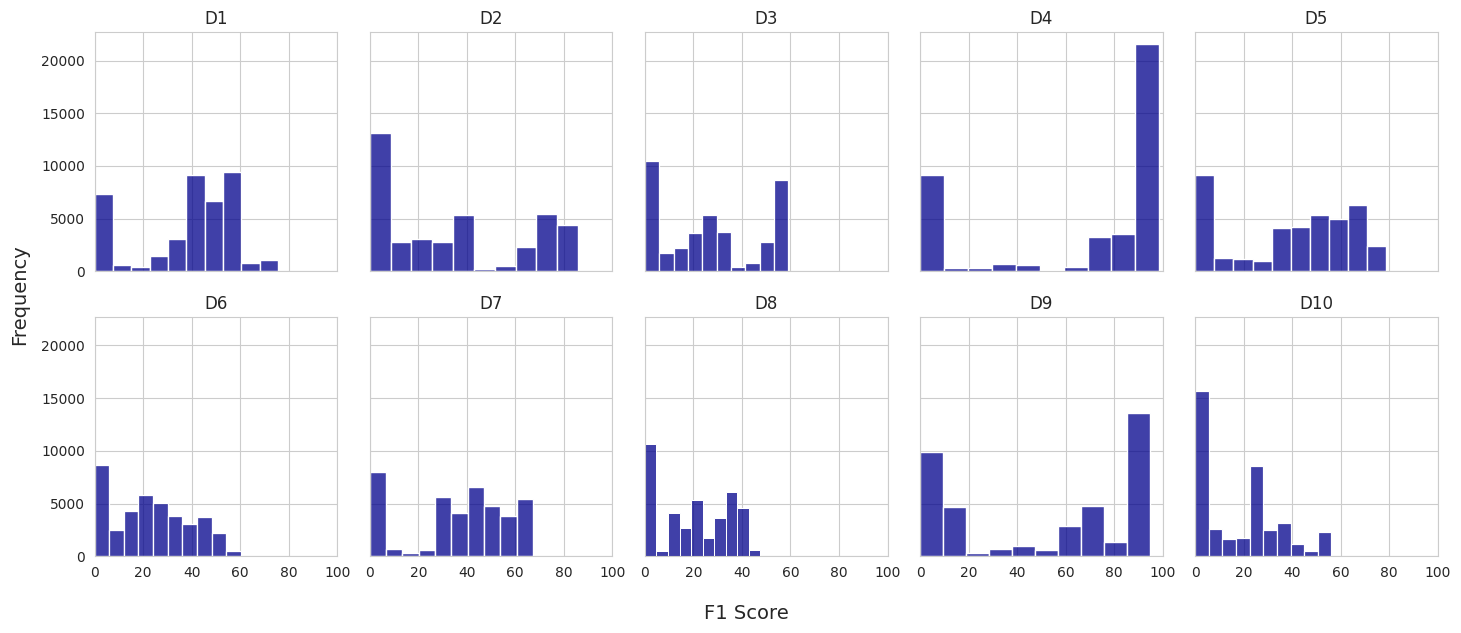
\includegraphics[width=0.97\linewidth]{Nikoletos-paper/figures/predictions/f1_score_distribution.png}
    % \vspace{-10pt}
    \caption{The distribution of F1-scores for the end-to-end ER pipeline of Figure~\ref{fig:eeter_pipeline}, when applying the 39,900 different configurations of Table~\ref{tab:parameter-values} to the 10 real-world datasets of Table~\ref{tab:dataset-specs}.}
    \label{fig:f1_boxplot_all}
    % \vspace{-14pt}
\end{figure*}

This is illustrated in Figure \ref{fig:f1_boxplot_all}, which demonstrates the range of F1 scores over 10 established real-world datasets 
%in Table \ref{tab:dataset-specs} 
(see Section \ref{sec:expSetup} for more details). {There is a separate diagram (i.e., bar chart) for each dataset. In each bar chart, the horizontal axis corresponds to the F-Measure of 
%For each dataset, we assessed the performance of 
the state-of-the-art end-to-end ER pipeline in Figure \ref{fig:eeter_pipeline} \cite{DBLP:journals/pvldb/ZeakisPSK23}, while the vertical axis corresponds to the frequency of the respective interval of F1 scores. This frequency stems from the grid search we applied to the configuration parameters of the selected ER pipeline: as shown in Table~\ref{tab:parameter-values}, grid search yields 39,900 different configurations (see Section \ref{sec:eteer_pipeline} for more details). Thus, there are 39,900 F1 scores per dataset, with their distribution illustrated through the bar charts.
%In fact, there is a separa we applied  . In total, we applied 39,900 different configurations per dataset, with 
We observe that} their performance exhibits a large deviation between the maximum and the minimum F1 score: 
in most datasets, the vast majority of configurations covers all values in $[0,50]$, while in datasets $D_4$ and $D_9$, the range is even larger, going up to 100 (both datasets contain unambiguous bibliographic data like author names and publication titles that ensure high performance for a large portion of configurations). This indicates significant sensitivity to the configuration parameters of the ER pipeline, with most options typically leading to rather low effectiveness. 

These settings highlight the importance of fine-tuning end-to-end ER pipelines. However, choosing the right configuration is a non-trivial task that requires time-consuming trial-and-error experimentations even for experts. To address this problem, we formulate parameter fine-tuning as a regression task over a large search space and leverage established sampling-based techniques for hyperparameter optimization. We experimentally demonstrate that these techniques are able to propose parameter configurations that approximate the optimal performance by curtailing the search space by orders of magnitude -- with fewer than 100 trials.

{
Note that the need for configuration fine-tuning applies also to the latest works on ER, which leverage LLMs for Entity Matching. In fact, LLM-based Matching comes in various forms that range from zero- and few-shot prompts \cite{DBLP:conf/edbt/PeetersSB25}, to SELECT prompts \cite{DBLP:conf/coling/WangCLCHSWZ25} and fine-tuning \cite{DBLP:journals/corr/abs-2409-08185}. These solutions involve numerous parameters (e.g., the selection criteria for the examples in few-shot prompting or fine-tuning), but apply only to the Verification part of end-to-end ER solutions (see Figure \ref{fig:eeter_pipeline}). This means that they disregard the preceding step of Filtering, which has a decisive impact on the candidate pairs processed by the matching algorithm. Most importantly, there is no clear winner among the plethora of proposed solutions (e.g., there is no comparison between the SELECT prompts and the fine-tuned LLMs), while their use in practice is quite challenging \cite{DBLP:conf/edbt/PeetersSB25,DBLP:conf/coling/WangCLCHSWZ25,DBLP:journals/corr/abs-2409-08185}: they have considerable hardware requirements, typically running on top of GPUs equipped with large VRAM, with their time efficiency being very low (i.e., high run-times). For these reasons, we exclusively consider the pipeline in Figure \ref{fig:eeter_pipeline}, which balances high effectiveness with high time efficiency by leveraging one of the top-performing pre-trained language models \cite{DBLP:journals/pvldb/ZeakisPSK23}.
}

%that are aware of the ground truth. 
Another obstacle in practical ER applications is the lack of ground truth with correct matches that allows for
%setting, though, the end user does not have a ground truth of (otherwise, the ER problem is solved/not needed for that dataset) so they cannot even 
evaluating the performance of different configurations automatically.
%, i.e., without costly
%, other than a brief and unreliable 
%manual inspections. 
%In the context of PPC's digital transformation, one of the main targets is the transition from legacy systems to high-end information systems such as ERP, CRMs etc. This requires deduplicating a series of databases that contain customer, employee and supplier data and were kept isolated in different departments. This data, though valuable, exhibit high levels of noise and of missing values, even identification attributes like person Ids. To leverage this legacy data, we need to democratize ER by enabling data scientists of any experience, even novice ones, to apply effective end-to-end ER pipelines. This can be accomplished by automating the parameter configuration of ER pipelines. 
%To this end, 
To address this task, we formulate a regression task, where the input comprises a feature vector describing the combination of a dataset and an ER pipeline configuration, while the output is the corresponding F1 score. In this context, datasets with known ground truth act as training instances, while datasets without a ground truth form the testing instances. We apply the trained model to all instances of a dataset without a ground truth and the one maximizing the expected F1 score indicates the most suitable parameter configuration. Using the end-to-end ER pipeline of Figure \ref{fig:eeter_pipeline}, we apply existing techniques for each part of this regression model: feature engineering is based on dataset profiling, the instances are generated by grid search, sampling-based algorithms, or both, and the learning process is carried out by two established approaches with integrated feature selection, namely Random Forests and AutoML. Our extensive experimental evaluation demonstrates which combination of these techniques yields the best performance.
%in terms of effectiveness and time efficiency.
%By estimating the 
%propose an auto-configurable ER pipeline that receives as input a dataset, optionally along with a partial ground truth of correct matches, 
%very small number of labeled matches, 
%and returns ER results after automatically deciding which configurations
%setting 
%are the most suitable for the task at hand.
%dataset. 
%Internally, our approach leverages a state-of-the-art end-to-end ER pipeline that uses language models for blocking and matching \cite{DBLP:journals/pvldb/ZeakisPSK23}. Its configuration parameters include the number of candidates per entity, the language model that creates the embedding vector of each entity, the clustering algorithm and the similarity threshold. Using a training set extracted from real datasets with a complete ground truth, AutoER applies AutoML techniques 
%or individual regression algorithms 
%to fine-tune these four parameters by selecting the best value in their domain.
%one among XXXXX different configurations. 
%We experimentally show that in almost all cases, AutoER yields results that are very close to the best obtainable ones, as they are determined via grid search over a large configuration space.

In summary, this works makes the following contributions:
%of this work are the following: 
\begin{itemize}[leftmargin=*]
    \item We define two problems for the automatic configuration of end-to-end ER pipelines: one assuming a ground truth and another one assuming no ground truth information. {To the best of our knowledge, there is no prior definition of relevant problems in ER literature.}
    \item We show how both problems can be addressed by existing techniques that have never been applied to the task of automatic ER pipeline configuration. {In fact, we are the first to apply sampling techniques to address the ground truth-aware auto-configuration problem, evaluating their relative performance in the context of ER. Note that ER differs from other learning tasks as it is impossible to materialize all negative instances (i.e., non-matching pairs), due to their quadratic space complexity. For this reason, the performance of the sampling techniques is exclusively guided by the F-Measure of the entire end-to-end ER pipeline. We are also the first to 
    model the regression-based solution to the ground truth-agnostic auto-configuration problem. We combine existing features with new ones in the feature engineering part of our solution, while exploring a rich diversity of strategies for instance generation. }
    %propose AutoER, a framework that solves both problems by automatically configuring a state-of-the-art end-to-end ER pipeline leveraging language models for blocking and matching. %based on  predicts the best ER pipeline configurations for a given dataset, with or without a known ground truth.
    %\item AutoER can operate even without a ground truth, but it can also exploit a small set of labeled matches and quickly find the best configuration. 
    \item We perform extensive experimental evaluations over 11 established, real-world datasets 
    %with real data 
    to identify the best solutions per problem.
    %demonstrates the high performance of our approaches in both problems
    %39,900 possible configurations generated by grid-search in 10 established datasets. including Z language models, ... , and YYY widely used datasets,} compared against state-of-the-art methods. 
    %\item 
\end{itemize}

We have open-sourced our code with a permissive license on Github: \underline{https://github.com/AI-team-UoA/AutoER}.
